\scanpage{47}
\mspage{\handwritten{15}}
a flat $\handwritten{\mathcal{O}}_S$-Module $\handwritten{\unsure{\mathcal{A}|a}}$ , and $\handwritten{\mathcal{E}}$ a quasi-coherent $\handwritten{\mathcal{O}}_S$-Module. We assume either that $G$ is affine\inserted{\handwritten{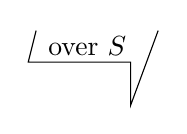
\begin{tikzpicture}[x=1cm,y=1cm,baseline=(n.base)]\node (n) at (0,0) {over $S$};\draw (-.65,.2)--(-.75,-.2)--(.55,-.2)--(.55,-.75)--(.9,.2);\end{tikzpicture}}}, or that \deleted{\unsure{G an}}d $\handwritten{\mathcal{E}}$ \deleted{are}\handwritten{is} flat\deleted{s} over $S$. Let $\handwritten{\rho:\mathcal{E}\to\mathcal{A}\otimes\mathcal{E}}$ be a homomorphism defining an ac-\linebreak tion of $G$ on $\handwritten{\mathcal{E}}$. Let $\handwritten{\mathcal{E}}_{\unsure{o|0}}$ be a quasi-coherent sub-$\handwritten{\mathcal{O}}_S$-Module of $\handwritten{\mathcal{E}}$ such that the homomorphism $\handwritten{\mathcal{E}}_{\unsure{o|0}}\handwritten{\longrightarrow\mathcal{A}\otimes\mathcal{E}}$ deduced from $\handwritten{\rho}$ factors through the canonical homomorphism \handwritten{(}injective\inserted{\handwritten{, thanks to the 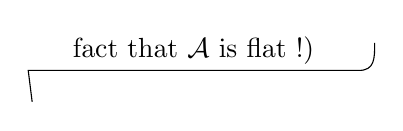
\begin{tikzpicture}[x=1cm,y=1cm,baseline=(n.base)]\node (n) at (0,0) {fact that $\mathcal{A}$ is flat !)};\draw (-2.05,-.65)--(-2.1,-.25)--(2.1,-.25) .. controls (2.3,-.25) and (2.3,-.1) .. (2.3,.1);\end{tikzpicture}}} $\handwritten{\mathcal{A}\otimes\mathcal{E}_{\unsure{o|0}}\longrightarrow\mathcal{A}\otimes\mathcal{E}}$ by means of the homomorphism $\handwritten{\rho_{\unsure{o|0}}:\mathcal{E}_{\unsure{o|0}}\longrightarrow\mathcal{A}\otimes\mathcal{E}_{\unsure{o|0}}}$. Then $\handwritten{\rho_{\unsure{o|0}}}$ defines an action of $G$ on $\handwritten{\mathcal{E}_{\unsure{o|0}}}$\handwritten{(},\handwritten{(} which we shall call the \uline{induced action} on $\handwritten{\mathcal{E}}_{\unsure{o|0}}$ by $\handwritten{\rho}$, and we shall say that $\handwritten{\mathcal{E}}_{\unsure{o|0}}$ is \uline{stable} under $\handwritten{\rho)}$.

This follows immediately from the definitions and from (11.\handwritten{6}). We shall note however that in general the canonical map $\handwritten{\mathbb{W}}(\handwritten{\mathcal{E}}_{\unsure{o|0}})\handwritten{\longrightarrow\mathbb{W}}(\handwritten{\mathcal{E}})$ is not injective.

\uline{Lemma 11.8.}- \uline{Let $G$ be a quasi-separated and quasi-compact $S$-group over $S$ such that $\handwritten{\mathcal{A}}(G)$ is a free $\handwritten{\mathcal{O}}_{\unsure{\mathbb{S}|S}}$-Module \deleted{\unsure{flat} $\handwritten{\mathcal{A}}$,} $\handwritten{\mathcal{A}}$ with basis $(\handwritten{\varphi}_i)$, $\handwritten{\mathcal{E}}$ a quasi-coherent $\handwritten{\mathcal{O}}_S$-Module. We assume either that $G$ is affine\inserted{\handwritten{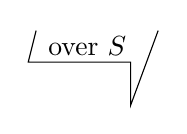
\begin{tikzpicture}[x=1cm,y=1cm,baseline=(n.base)]\node (n) at (0,0) {over $S$};\draw (-.65,.2)--(-.75,-.2)--(.55,-.2)--(.55,-.75)--(.9,.2);\end{tikzpicture}}}, or that $G$ and $\handwritten{\mathcal{E}}$ are flat over $S$. Let $\handwritten{\rho:\mathcal{E}\to\mathcal{A}\otimes\mathcal{E}}$ be a homomorphism defin-\linebreak ing an action of $G$ on $\handwritten{\mathcal{E}}$, and let $x\handwritten{\in\Gamma}(S,\handwritten{\mathcal{E}})$. Put $\handwritten{\rho}(x)=\handwritten{\sum\varphi}_i\handwritten{\otimes x}_i$, where the $x_i\handwritten{\in\Gamma}(S,\handwritten{\mathcal{E}})$ are uniquely determined by this relation). Then the submodule\inserted{\handwritten{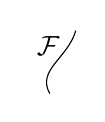
\begin{tikzpicture}[x=1cm,y=1cm,baseline=(n.base)]\node (n) at (0,0) {$\mathcal{F}$};\draw (.35,.2) .. controls (.25,-.15) and (-.15,-.3) .. (.02,-.6);\end{tikzpicture}}} of $\handwritten{\mathcal{E}}$ generated by the $x_i$ is stable under $\handwritten{\rho}$,\deleted{and contains $x$.}\inserted{quasi-coherent} and of finite type over $\handwritten{\mathcal{O}}_S$, and $x\handwritten{\in\Gamma}(S,\handwritten{\mathcal{F}})$.}
\figure{\handwritten{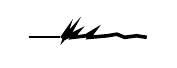
\begin{tikzpicture}[x=1cm,y=1cm]\draw[line width=.7pt] (0,0) -- (.4,0);\draw[line width=1.3pt] (.42,-.01) -- (.49,.09) -- (.46,0) -- (.55,.1) -- (.5,.01) -- (.62,.07) -- (.56,0) -- (.73,.02) -- (.83,.08) -- (.77,0) -- (1,.02) -- (1.12,.04) -- (1.22,0) -- (1.37,.02) -- (1.5,0);\end{tikzpicture}}}

\deleted{Let $\handwritten{\mathcal{F}}$ be the submodule of $\handwritten{\mathcal{E}}$ generated by the $x_i$\unsure{,|.}} \handwritten{I}t is clear that $\handwritten{\mathcal{F}}$ is quasi-coherent and of finite type. Axiom (CM1) shows that $\handwritten{\sum\Delta}(\handwritten{\varphi}_i)\handwritten{\otimes}x_i=\handwritten{\sum\varphi}_i\handwritten{\otimes\rho}(x_i)$ ; on the other hand, $\handwritten{\Delta(\varphi}_i\handwritten{)=\sum\varphi}_j\handwritten{\otimes}a_{ij}$ , whence $\handwritten{\sum\varphi}_j\handwritten{\otimes}a_{ij}\handwritten{\otimes}x_i=\handwritten{\sum\varphi}_i\handwritten{\otimes\rho}(x_i)$, whence, since the $\handwritten{\varphi}_i$ form a basis of $\handwritten{\mathcal{A}}$, $\handwritten{\rho}(x_i)=\handwritten{\sum}a_{ji}\handwritten{\otimes}x_{\handwritten{i}}$, where $a_{ji}\handwritten{\in\Gamma}(S,\handwritten{\mathcal{A}})$, which shows that $\handwritten{\rho(\mathcal{F})\subset\mathcal{A}\otimes\mathcal{F}}$, hence $\handwritten{\mathcal{F}}$ is stable under $\handwritten{\rho}$. Finally axiom (CM2) shows that $x=\handwritten{\sum_i\eta}(\handwritten{\varphi}_i)x_i\handwritten{\in\Gamma}(S,\handwritten{\mathcal{F}})$.

\uline{Proposition 11.9.- Let $G$ be a quasi-compact quasi-separated $S$-group over $S$ such that $\handwritten{\mathcal{A}}=\handwritten{\mathcal{A}}(G)$ be-\linebreak comes locally free after a faithfully flat quasi-compact extension of the base $S$ (which} is the case\inserted{\handwritten{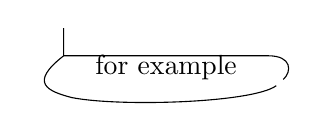
\begin{tikzpicture}[x=1cm,y=1cm,baseline=(n.base)]\node (n) at (0,0) {for example};\draw (-1.3,.5)--(-1.3,.15) .. controls (-1.75,-.2) and (-1.5,-.3) .. (-1.2,-.38) .. controls (-.6,-.5) and (1.1,-.45) .. (1.4,-.23);\draw (-1.3,.15)--(1.3,.15) .. controls (1.6,.15) and (1.6,-.05) .. (1.49,-.15);\end{tikzpicture}}} when $G$ is a reductive group, as we\deleted{\unsure{it}} shall see in \deleted{the lecture} \handwritten{$\overline{\underline{\mathrm{XXV}}}$}), \uline{and} \uline{let $\handwritten{\mathcal{E}}$ be a quasi-coherent $\handwritten{\mathcal{O}}_S$-\deleted{module}\handwritten{Module} . We assume either that $G$ is affine\inserted{\handwritten{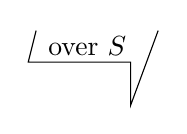
\begin{tikzpicture}[x=1cm,y=1cm,baseline=(n.base)]\node (n) at (0,0) {over $S$};\draw (-.65,.2)--(-.75,-.2)--(.55,-.2)--(.55,-.75)--(.9,.2);\end{tikzpicture}}}, or that $G$ and $\handwritten{\mathcal{E}}$ are flat over $S$. Let $\handwritten{\rho:\mathcal{E}\longrightarrow\mathcal{A}\otimes\mathcal{E}}$ be a homomorphism defining an action of $G$ on $\handwritten{\mathcal{E}}$.}
% archive sheet number: 46
